\tikzset{overlap/.style={fill=yellow!30},
    block wave/.style={thick},
    function f/.style={block wave, red!50},
    function g/.style={block wave, green!50},
    convolution/.style={block wave, blue!50},
    function g position/.style={function g, dashed, semithick},
    major tick/.style={semithick},
    axis label/.style={anchor=west},
    x tick label/.style={anchor=north, minimum width=7mm},
    y tick label/.style={anchor=east},
}

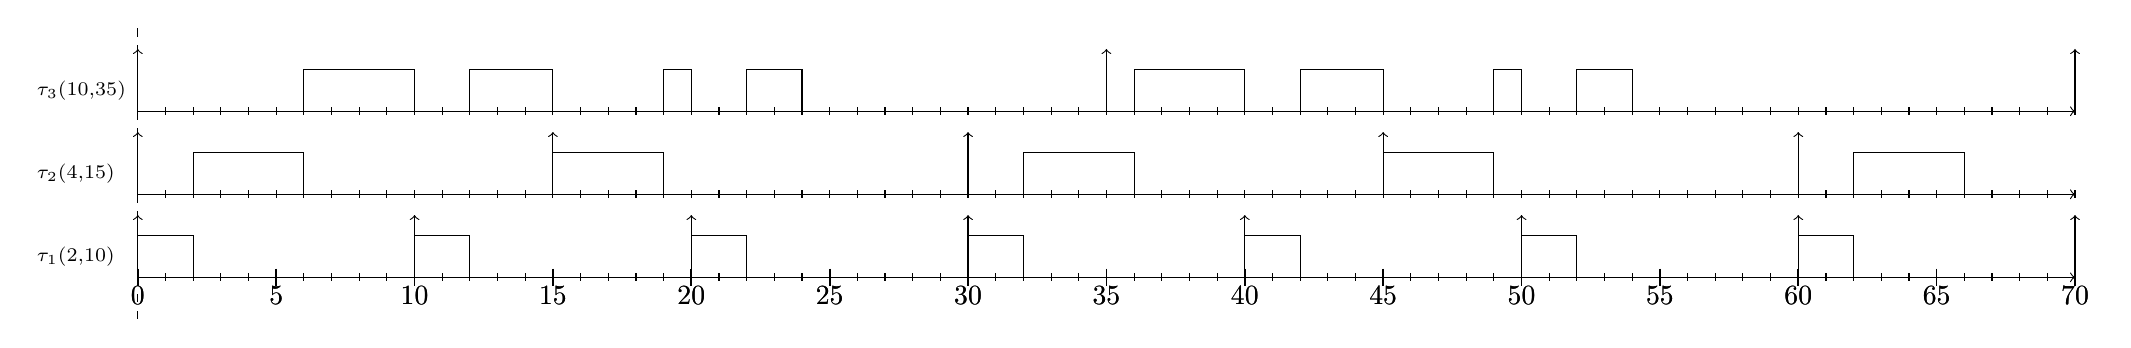
\begin{tikzpicture}[x=1em, y=1.5em]

	%
	\draw[->] (0, 0) -- (70, 0);
	\draw[->] (0, 2) -- (70, 2);
	\draw[->] (0, 4) -- (70, 4);
	% Small tickmarks on the x axis
        	\foreach \x in {0, 1,...,70} {
            		\draw (\x, 0.1) -- (\x, -0.1);
        	}
        	\foreach \x in {0, 1,...,70} {
            		\draw (\x, 2+0.1) -- (\x, 2+-0.1);
        	}
        	\foreach \x in {0, 1,...,70} {
            		\draw (\x, 4+0.1) -- (\x, 4+-0.1);
        	}
        % Labels on the $x$ axis; the llap makes the label center on the
        % number without the minus.
        \foreach \x / \label in {0, 5, ..., 70, 0, 5, ..., 70} {
            \node[x tick label] at (\x, 0) {$\label$};
            \draw[major tick] (\x, 0.2) -- (\x, -0.2);
        }

        \node[axis label] at (-4,0.5) {$\scriptstyle \tau_1(2, 10)$};
        \node[axis label] at (-4,2+0.5) {$\scriptstyle \tau_2(4, 15)$};
        \node[axis label] at (-4,4+0.5) {$\scriptstyle \tau_3(10, 35)$};
	% start
	\draw[dashed] (0, -1) -- (0, 6);
	
	% periodic
		% job 1 (2, 10)
		\draw[->] (0, 0) -- (0, 1.5);
		\draw[->] (10, 0) -- (10, 1.5);
		\draw[->] (20, 0) -- (20, 1.5);
		\draw[->] (30, 0) -- (30, 1.5);
		\draw[->] (40, 0) -- (40, 1.5);
		\draw[->] (50, 0) -- (50, 1.5);
		\draw[->] (60, 0) -- (60, 1.5);
		\draw[->] (70, 0) -- (70, 1.5);
		% job 2 (4, 15)
		\draw[->] (0, 2) -- (0, 3.5);
		\draw[->] (15, 2) -- (15, 3.5);
		\draw[->] (30, 2) -- (30, 3.5);
		\draw[->] (45, 2) -- (45, 3.5);
		\draw[->] (60, 2) -- (60, 3.5);
		% job 3 (10, 35)
		\draw[->] (0, 4) -- (0, 5.5);
		\draw[->] (35, 4) -- (35, 5.5);
		\draw[->] (70, 4) -- (70, 5.5);
	% interval
		% job 1
		\draw (0, 0) rectangle (2, 1);
		\draw (10, 0) rectangle (12, 1);
		\draw (20, 0) rectangle (22, 1);
		\draw (30, 0) rectangle (32, 1);
		\draw (40, 0) rectangle (42, 1);
		\draw (50, 0) rectangle (52, 1);
		\draw (60, 0) rectangle (62, 1);
		% job 2
			% first
		\draw (2, 2) rectangle (6, 3);
		\draw (15, 2) rectangle (19, 3);
			% second
		\draw (32, 2) rectangle (36, 3);
		\draw (45, 2) rectangle (49, 3);
		\draw (62, 2) rectangle (66, 3);
		% job 3
			% first
		\draw (6, 4) rectangle (10, 5);
		\draw (12, 4) rectangle (15, 5);
		\draw (19, 4) rectangle (20, 5);
		\draw (22, 4) rectangle (24, 5);
			% second
		\draw (36, 4) rectangle (40, 5);
		\draw (42, 4) rectangle (45, 5);
		\draw (49, 4) rectangle (50, 5);
		\draw (52, 4) rectangle (54, 5);
\end{tikzpicture}